\documentclass[tikz,border=8pt]{standalone}
% Shared look for every TikZ diagram. Load with \input{../../tools/tikz-style.tex}
\usepackage[sfdefault]{roboto}
\usetikzlibrary{arrows.meta, positioning, shapes.geometric, calc, fit, backgrounds}
\definecolor{cblue}{HTML}{4C78A8}
\definecolor{corange}{HTML}{F58518}
\definecolor{cgreen}{HTML}{54A24B}
\definecolor{cred}{HTML}{E45756}
\definecolor{cpurple}{HTML}{B279A2}
\definecolor{cgrey}{HTML}{6B6B6B}
\tikzset{
  every picture/.style={font=\sffamily, line width=1.2pt},
  box/.style={draw=#1, fill=#1!12, rounded corners=4pt, align=center, inner sep=7pt, minimum height=1.1cm},
  box/.default=cgrey,
  arrow/.style={-{Stealth[length=3mm]}, draw=cgrey, line width=1.4pt},
  title/.style={font=\sffamily\bfseries\Large},
  note/.style={font=\sffamily\small, text=cgrey, align=center},
}
\AtBeginDocument{\hyphenpenalty=10000 \exhyphenpenalty=10000}

% The rear axle runs inside the front axle on a curve. With the front axle on the 10 m arc, the rear axle, square to
% the radius at its own point, is at sqrt(10^2 - 2.5^2) = 9.682 m from the centre: 0.318 m inside. Drawn not to scale
% (arc radius 5 units, wheelbase 2.5 units) so that the gap shows; the numbers are for the real car.
\begin{document}
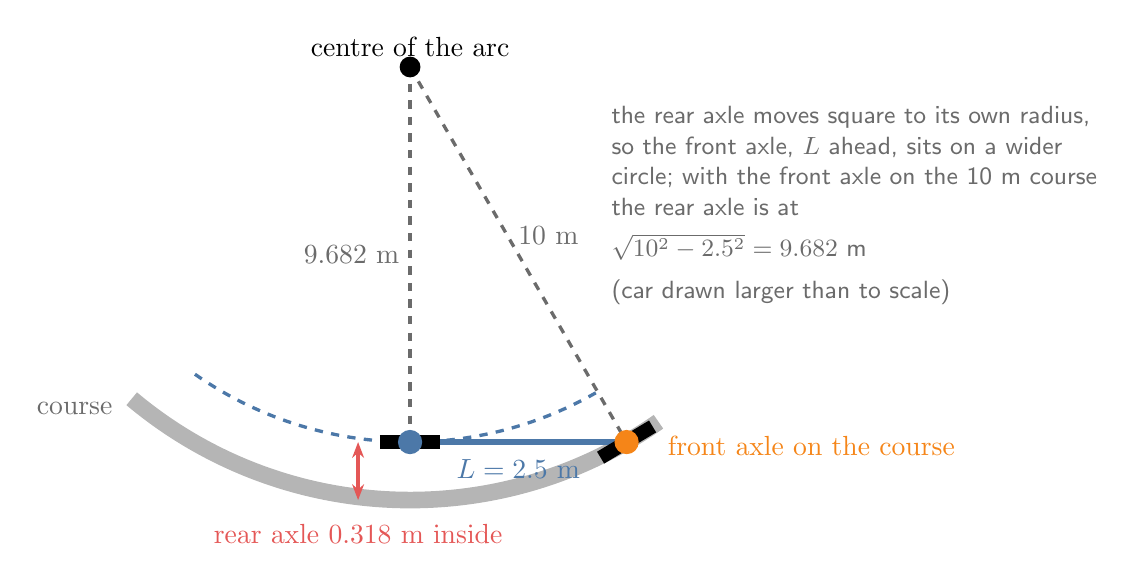
\begin{tikzpicture}[every node/.append style={font=\normalsize}, x=1.1cm, y=1.1cm]
  \coordinate (C) at (0,0);
  \coordinate (Rr) at (0,-4.330);
  \coordinate (F) at (2.5,-4.330);
  \draw[cgrey!50, line width=6pt] (230:5) arc (230:305:5);
  \node[cgrey, anchor=east] at (230:5.15) {course};
  \draw[cblue, line width=1.2pt, dashed] (235:4.33) arc (235:300:4.33);
  \draw[cgrey, line width=1.2pt, dashed] (C) -- node[left, pos=0.5] {9.682 m} (Rr);
  \draw[cgrey, line width=1.2pt, dashed] (C) -- node[right, pos=0.45] {10 m} (F);
  \draw[cblue, line width=2pt] (Rr) -- node[below=2pt] {$L = 2.5$ m} (F);
  \draw[black, line width=5pt] (-0.35,-4.330) -- (0.35,-4.330);
  \draw[black, line width=5pt] ($(F)+(-0.30,-0.18)$) -- ($(F)+(0.30,0.18)$);
  \fill[cblue] (Rr) circle (0.14); \fill[corange] (F) circle (0.14);
  \node[corange, anchor=west] at ($(F)+(0.35,-0.05)$) {front axle on the course};
  \draw[cred, line width=1.4pt, {Stealth[length=2mm]}-{Stealth[length=2mm]}] (-0.6,-4.330) -- (-0.6,-5);
  \node[cred, anchor=north] at (-0.6,-5.15) {rear axle 0.318 m inside};
  \fill[black] (C) circle (0.12);
  \node[anchor=south] at (C) {centre of the arc};
  \node[note, anchor=west, text width=6.2cm, align=left] at (2.2,-1.6) {the rear axle moves square to its own radius, so the front axle, $L$ ahead, sits on a wider circle; with the front axle on the 10~m course the rear axle is at\\[4pt] $\sqrt{10^2 - 2.5^2} = 9.682$ m\\[4pt] (car drawn larger than to scale)};
\end{tikzpicture}
\end{document}
